\documentclass{article}

% use option titlepage to get the title on a page of its own.
\usepackage{tikz}

\usetikzlibrary{shapes.geometric, arrows}

\tikzstyle{startstop} = [rectangle, minimum width=2cm, minimum height=2cm,text centered, draw=black, fill=red!30]
\tikzstyle{process} = [circle, minimum width=2cm, minimum height=2cm, text centered, draw=black, fill=orange!30]
\tikzstyle{decision} = [diamond, minimum width=2cm, minimum height=2cm, text centered, draw=black, fill=green!30]
\tikzstyle{io} = [rectangle, minimum width=2cm, minimum height=1cm, text centered, draw=black, fill=blue!30]
\tikzstyle{arrow} = [thick,->,>=stealth]

\usepackage{authblk}

\title{Genetic Programming Video Games}

\author{Sean Butler}
\affil{Department of Computer Science and Creative Technology, \\ Faculty of Engineering and Technology, \\ UWE, Bristol. UK.}
\date{2020 August}


\begin{document}

\maketitle

\section{Introduction}

\paragraph{} Lorem ipsum dolor sit amet, consectetur adipiscing elit, sed do eiusmod tempor incididunt ut labore et dolore magna aliqua. Ut enim ad minim veniam, quis nostrud exercitation ullamco laboris nisi ut aliquip ex ea commodo consequat. Duis aute irure dolor in reprehenderit in voluptate velit esse cillum dolore eu fugiat nulla pariatur. Excepteur sint occaecat cupidatat non proident, sunt in culpa qui officia deserunt mollit anim id est laborum.

\section{Method}

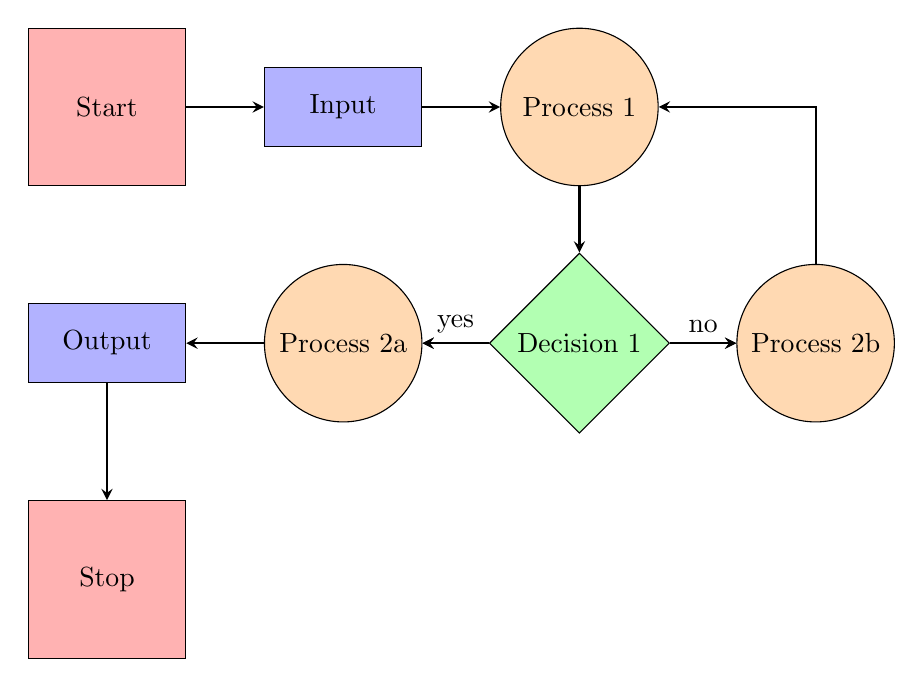
\begin{tikzpicture}[node distance=3cm]
    \node (start) [startstop] {Start};
    \node (in1) [io, right of=start] {Input};
    \node (pro1) [process, right of=in1] {Process 1};
    \node (dec1) [decision, below of=pro1] {Decision 1};
    \node (pro2a) [process, left of=dec1] {Process 2a};
    \node (pro2b) [process, right of=dec1] {Process 2b};
    \node (out1) [io, left of=pro2a] {Output};
    \node (stop) [startstop, below of=out1] {Stop};
    \draw [arrow] (start) -- (in1);

    \draw [arrow] (in1) -- (pro1);
    \draw [arrow] (pro1) -- (dec1);
    \draw [arrow] (dec1) -- (pro2a);
    \draw [arrow] (dec1) -- (pro2b);
    \draw [arrow] (dec1) -- node[anchor=south] {yes} (pro2a);
    \draw [arrow] (dec1) -- node[anchor=south] {no} (pro2b);
    \draw [arrow] (pro2b) |- (pro1);
    \draw [arrow] (pro2a) -- (out1);
    \draw [arrow] (out1) -- (stop);

\end{tikzpicture}

\section{A Survey of Classic Era Arcade Games}

\paragraph{} Taken from (https://www.ranker.com/crowdranked-list/the-best-classic-arcade-games)
 site is a lost of the most popular arcade games from the classic era.
Though pretty much any list of popular arcade games from the era would do.

\begin{itemize}

    \item Galaga
    \item Donkey Kong
    \item Pac Man
    \item Space Invaders (1 and 4 are synonymous)
    \item Ms. Pac Man (3 and 5 are synonymous)
    \item Dig Dug
    \item Gauntlet
    \item Asteroids
    \item Mario Bros (not an arcade game, also covered elsewhere)
    \item 1942
    \item Defender
    \item Street Fighter II 
    \item Centipede
    \item Street Fighter
    \item Double Dragon (see 12 + 14)
    \item Joust
    \item Mortal Combat (see 12, 14 + 15)
    \item etc
    \item etc
    \item PONG
    \item SPY HUNTER

\end{itemize}

\paragraph{} Ignore the strolling beat em up fighting games like Street Fighter and etc. Also
ignore Mario Bros as really a console game. Both are well covered in other literature as well.

\section{Patterns Found Across Many Games}


\section{Game Patterns}

\section{Entity Patterns}

\paragraph{} These games all have the following patterns in common.

\begin{itemize}  
\item Player Can Move
\item Flat 2D Space (asteroids?!)
\item Either Player Reaches Goal To Win or Player Defeats (all) Enemies to Win
\item Enemies Hurt Player on Collision
\item More Enemies Than Players
\end{itemize}


\subsection{Common Patterns}

 - Some Environment Blocks are visible and impassible, if so then only small fraction of space
 - Player has 3 Health
 - Enemies have 1 Health
 - Players Shoot Hurtful Projectiles
 - Enemies Shoot Hurtful Projectiles
 - Waves of Enemies
 - Stationary Player Respawn (Start) Point


\subsection{Uncommon Patterns}

 - Some Environment Can be destroyed
   - if so then much more common
 - Player collects Items for Powers
   - Suppressed abilities, collectables unlock them
 - Enemies Grow or Space Shrinks either directly or indirectly (more on this later)
 - Enemies Reach Goal To Win (Player Lose)

\section{Criteria for Quality Arcade Games}

\subsection{Requirements / Must}
 
These can be coded into the wider system as they are necessary

 - Complete (win or lose) a Level in over 30 seconds
     - lets say @16fps 16*60*0.5 = about 500 moves
 - Must Complete (win or lose) a Level in under 5 minutes
     - lets say @16fps 16*60*5 = about 5000 moves
 - Cannot win just by staying still and waiting
    - Or moving to safe place and waiting

\subsection{Goals / Should}

 These can be set as evolutionary goals via fitness functions

 - Should Complete (win or lose) a Level in under 3 minutes
     - lets say @16fps 16 x 60 x 3 = about 3000 moves
     - lets say @16fps 16 x 60 x 5 = about 5000 moves
 - Player completes a Level a fraction (say, 1/2 ) of the time
    - Could be, given 3 hearts, lose 1 heart per level on average
 - Should Move over range of Locations
    - Simple Statistical Measure
 - Likely cover the same ground more than once
    - Simple Statistical Measure
 - Should interact (get close too) enemies to succeed

 - Enemy May sometimes Defeat Player by collision
 - Enemy Move towards and Away from the Player
 - Enemy Have Repetitive Behaviours which can be observed
 - Enemy Should interact (get close too) player at some point to succeed

 - Enemy Rewards the Player on its Death

\subsection{More Advanced Patterns}

\subsection{Environment Generation Strategies}

 - Use Randomised depth first search to carve out a maze
 - Randomly place few long walls
 - Randomly place single blocks

\subsection{Player Characteristics}

\subsection{Required Characteristics}

- Can perceive (nearly) the whole visible level, radius will do. Doesnt need to interrogate (say via ray casts). This is not a simulation the player sees the arena like a seagull or a drone. So can tell direction and distance to specific interesting elements like the goal once Goal has been onscreen Goal.
- Is movable

\subsection{Optional Characteristics}

- Reaches a Goal coords to win
- Has scalar health. WHen health reaches zero loses
- Has scalar points. Reaches a Score to win
- When low health finds and collects health
- Avoids Damage

\subsection{Enemy}

\subsection{Given/Unavoidable Characteristics}

- Has start/anchor point
    Set Anchor()

- Has limits/range/flaws to its perception

- Has limits/range to its movement
    If Distance From Anchor > Range

\subsection{Derived}

- Interacts with the Player at least once on a playthrough
- Hurts or Hinders the Player
- Rewards the Player on its Death
- Has predictable Repetitive Behaviour
- Vulnerable to Damage

\subsection{Goal}

Once entity has been in range of me they always know where I am.

\section{Door-Key Challenge}

\subsection{Door}

- Blocking and Changes to Passable
- Requires External Message
    - collection of pickups
    - killing of enemies
    - visit location
    - etc

Key

Arena



\blindtext
\end{document}

